In this section we present the results obtained for the SFs in the $Z\to\tauhad e$ and $Z\to\tauhad \mu$ final states. 
\subsection{Z-$\pt$ Study}
Since the events selected in this analysis are highly boosted $\Zll$ ones, the Z$\pt$ is expected to peak at higher values than for normal back to back $\Zll$ events. Previous results \cite{Aad:2019wmn}, have shown that different Monte Carlo generators predict different shapes for the Z$\pt$ distribution, specially in the high-$\pt$ tail. In this analysis, we used two different MC generators for the signal samples, $\POWPY[8]$ (PoPy) and $\SHERPA$. As can be seen in Fig. \ref{Fig10}, Sherpa does a better job describing the Z boson transverse momentum for high Z$\pt$ values than PoPy. However, both generators underestimate the measured value below the Z$\pt=300$ GeV region. 

Fig. \ref{Fig11}, shows the Z$\pt$ distribution for our final selected events. Looking at these plots, it is clear that $\Sherpa$ does a better job for highly-boosted $\Zll$ events. 

If we just measure the single ratio defined by equation \ref{eq14}, we would be sensitive to the Z$\pt$ miss-modelling. However, when taking the double ratio this effect should cancel. Additionally, the $Z\to\tauhad\taulep$ and $\Zll$ PoPy samples have been re-weighted according to the data/simulation ratio given in Fig. \ref{Fig10}. We call this samples PoPy-RW. The aim of this procedure is to show that the double ratio method is not sensitive at first order to the Z$\pt$ modelling.

\begin{figure}[htbp]
	\centering
	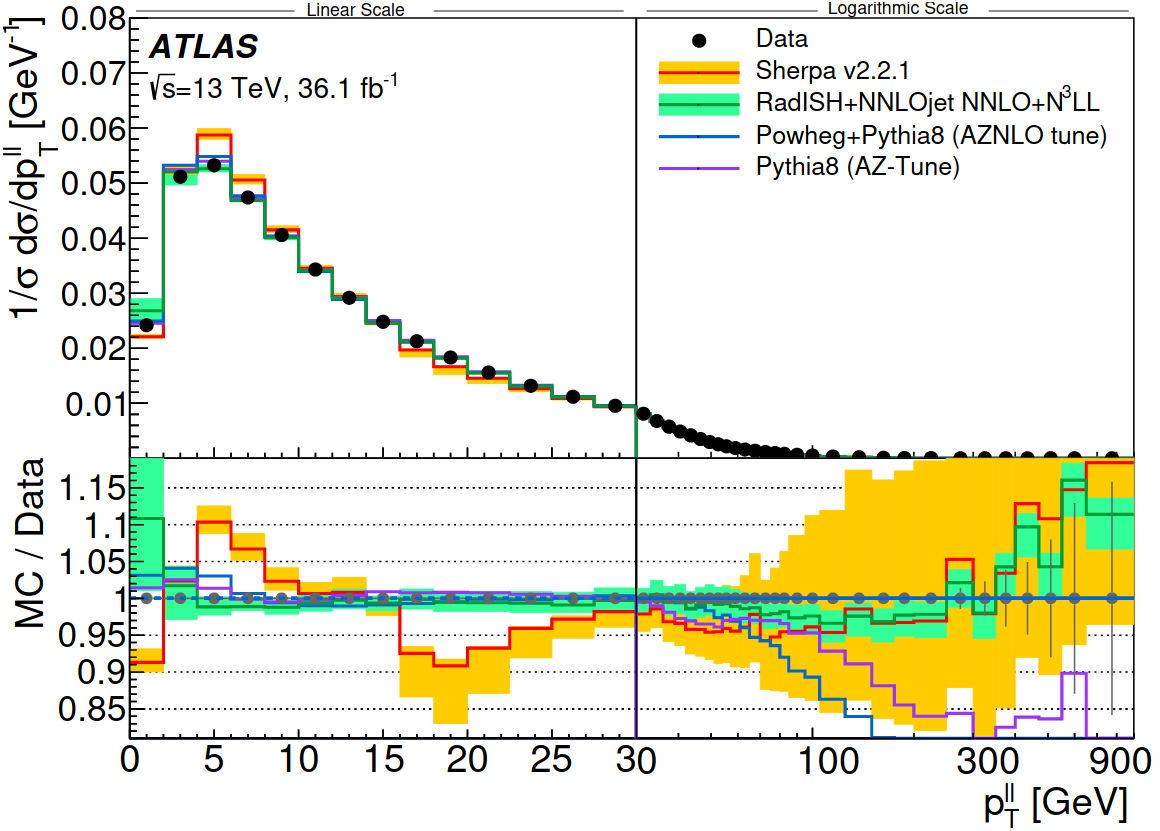
\includegraphics[width=0.6\textwidth]{figures/Fig10}
	\caption{Comparison of the Z$\pt$ modelling in Drell-Yan events made by different MC generators. Taken from \cite{Aad:2019wmn}}
	\label{Fig10}
\end{figure}

\begin{figure}[htbp]
	\centering
	\subfloat[]{\label{Fig11a}{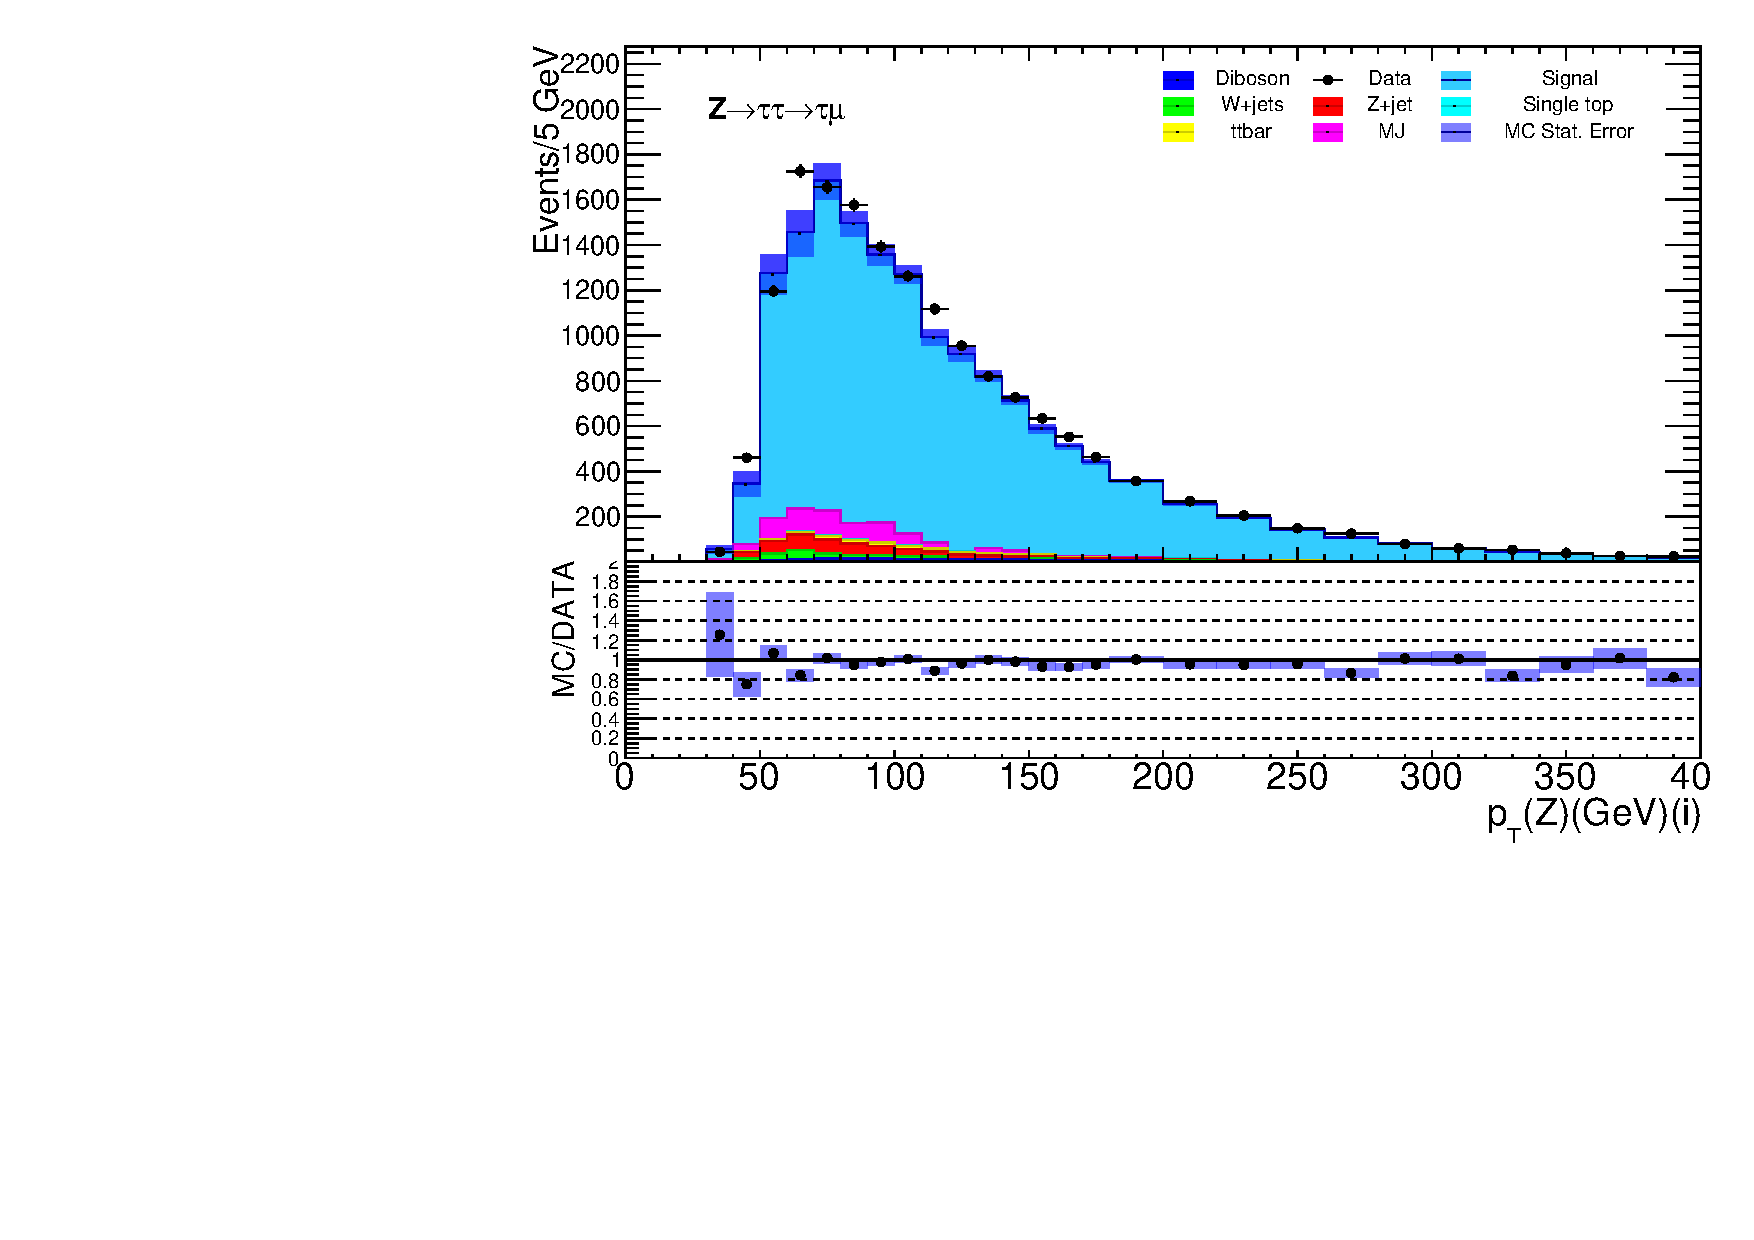
\includegraphics[width=0.50\textwidth]{figures/Fig11a}}}\hfill
	\subfloat[]{\label{Fig11b}{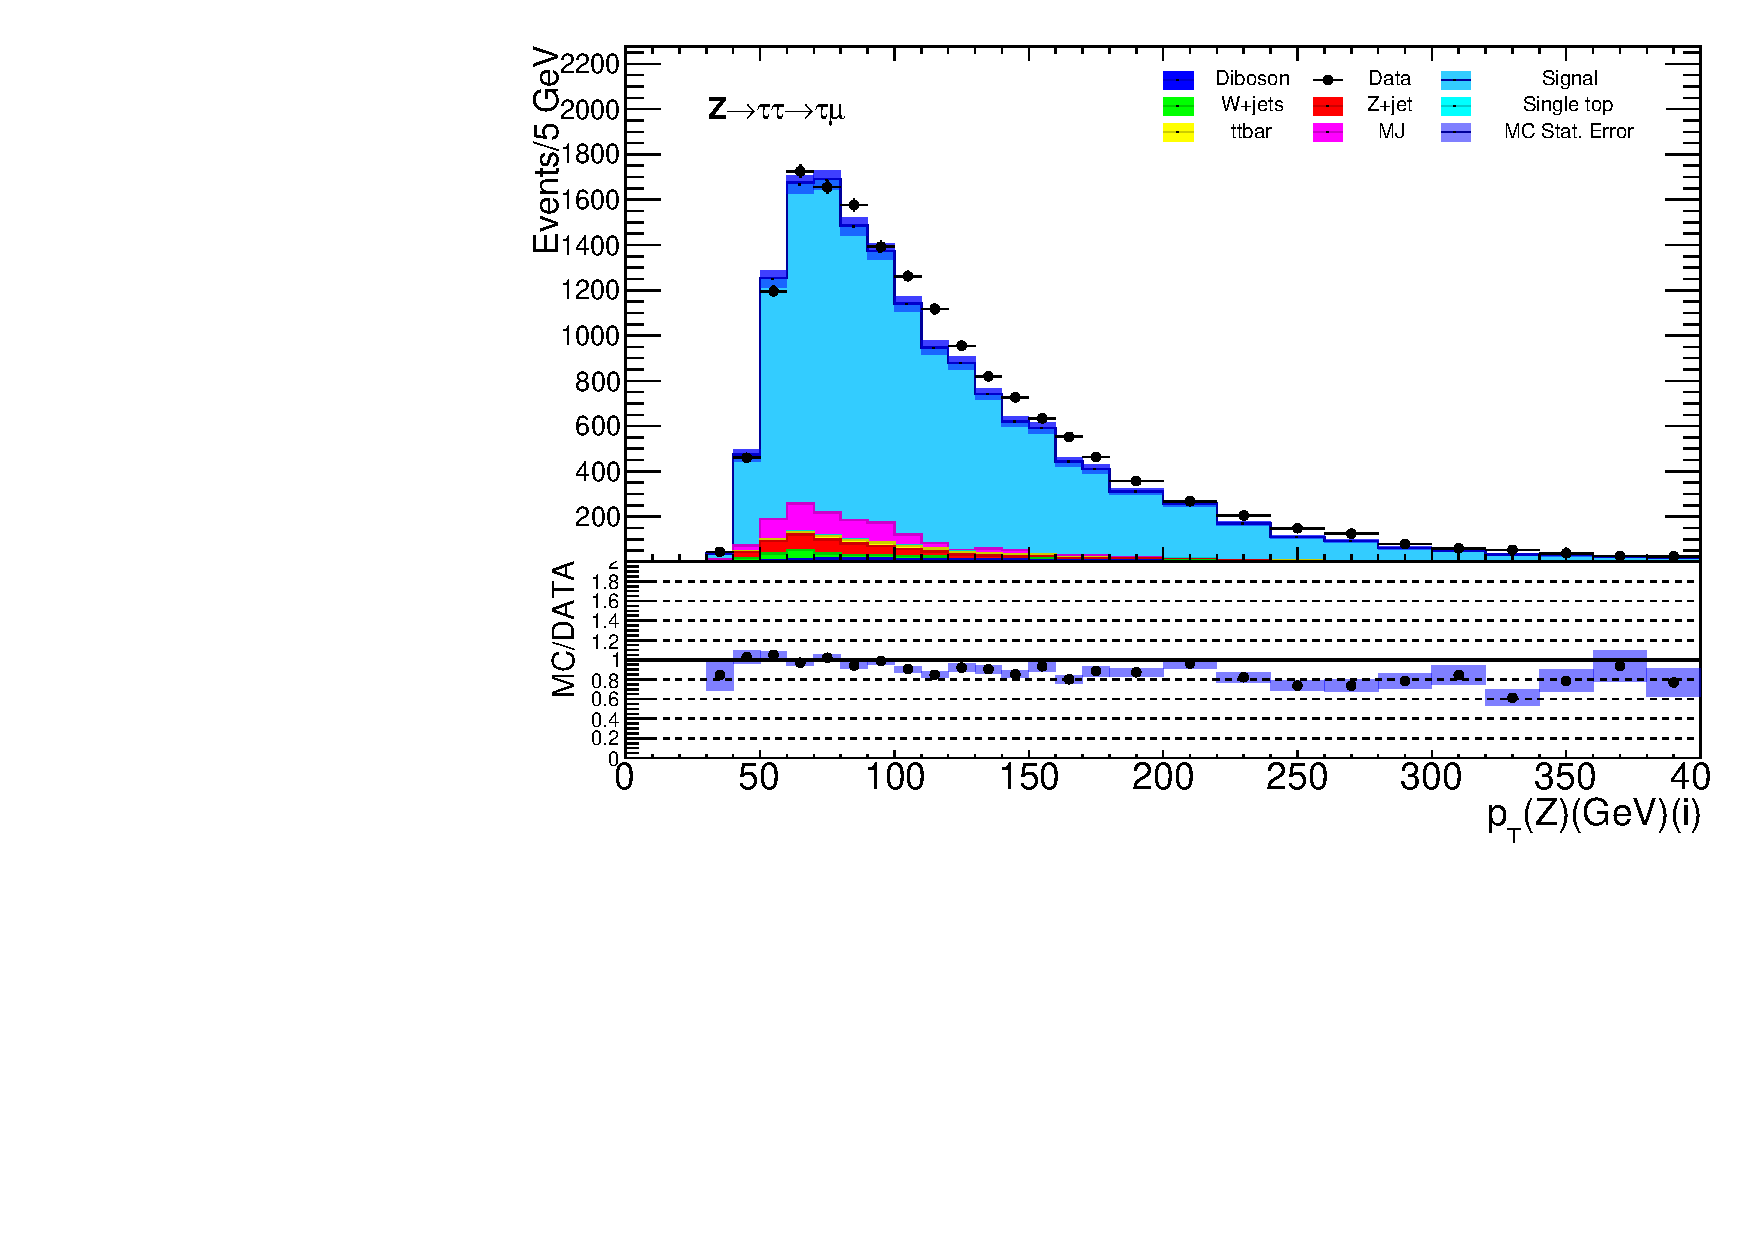
\includegraphics[width=0.50\textwidth]{figures/Fig11b}}}
	\caption{Z$\pt$ distributions for $Z\to\tauhad\mu$ events. $\Sherpa$ prediction (a) is much closer to the data. Meanwhile, (b) $\POWPY[8]$ tends to underestimate the data increasingly as the Z$\pt$ becomes higher. }
	\label{Fig11}
\end{figure}
\subsection{Scale Factors}
The total yields for all the final states, using Sherpa samples as signal, are shown in Table \ref{Tab6}. With these figures, we calculate the C factors and the SFs reported in the second column of Table \ref{Tab7} and \ref{Tab8}. The SFs obtained for the other MC generator configurations are in the two remaining columns. The values are reported as,
\begin{equation}
	\text{Central value}\pm\text{Uncorrelated Uncertainty}\pm\text{Correlated Uncertainty}=\text{Total}.
	\label{equncer}
\end{equation}
All the uncertainties reported in the tables are statistical uncertainties. They are split into two categories. First, uncorrelated uncertainties. These come from the MC statistical uncertainty on the signal sample and the MJBG contribution, since the latter is calculated taking into account the prediction for the signal in the control region. The correlated uncertainty, is coming from the data statistical uncertainties and the EWBG component. Those ones are common to any of the SFs quoted on Tables \ref{Tab6} and \ref{Tab7} for the same final states. This is the reason they should not be included when comparing different MC generators (different columns) and are called correlated. Finally, the total statistical uncertainty is calculated adding both correlated and uncorrelated components in quadrature. This value is the one that should be used to compare between different final states.
\begin{table}[]
	\resizebox{\textwidth}{!}{%
		\begin{tabular}{|
				>{\columncolor[HTML]{FFFFFF}}c 
				>{\columncolor[HTML]{FFFFFF}}c 
				>{\columncolor[HTML]{FFFFFF}}c 
				>{\columncolor[HTML]{FFFFFF}}c 
				>{\columncolor[HTML]{FFFFFF}}c 
				>{\columncolor[HTML]{FFFFFF}}c 
				>{\columncolor[HTML]{FFFFFF}}c |}
			\hline
			\multicolumn{1}{|c|}{\cellcolor[HTML]{FFFFFF}\textbf{Final State}}  & \multicolumn{2}{c|}{\cellcolor[HTML]{FFFFFF}\textbf{$Z\to\tauhad\mu$}}                                                              & \multicolumn{1}{c|}{\cellcolor[HTML]{FFFFFF}}                                        & \multicolumn{2}{c|}{\cellcolor[HTML]{FFFFFF}\textbf{$Z\to\tauhad e$}}                                                              & \cellcolor[HTML]{FFFFFF}                                     \\ \cline{1-3} \cline{5-6}
			\multicolumn{1}{|c|}{\cellcolor[HTML]{FFFFFF}\textbf{Sample}}       & \multicolumn{1}{c|}{\cellcolor[HTML]{FFFFFF}\textbf{1-Prong}}    & \multicolumn{1}{c|}{\cellcolor[HTML]{FFFFFF}\textbf{3-Prong}}    & \multicolumn{1}{c|}{\multirow{-2}{*}{\cellcolor[HTML]{FFFFFF}\textbf{$Z\to\mu\mu$}}} & \multicolumn{1}{c|}{\cellcolor[HTML]{FFFFFF}\textbf{1-Prong}}    & \multicolumn{1}{c|}{\cellcolor[HTML]{FFFFFF}\textbf{3-Prong}}    & \multirow{-2}{*}{\cellcolor[HTML]{FFFFFF}\textbf{$Z\to ee$}} \\ \hline
			\multicolumn{1}{|c|}{\cellcolor[HTML]{FFFFFF}\textbf{True Signal}}  & \multicolumn{1}{c|}{\cellcolor[HTML]{FFFFFF}$6083.19\pm61.147$}  & \multicolumn{1}{c|}{\cellcolor[HTML]{FFFFFF}$1587.927\pm32.098$} & \multicolumn{1}{c|}{\cellcolor[HTML]{FFFFFF}}                                        & \multicolumn{1}{c|}{\cellcolor[HTML]{FFFFFF}$4656.503\pm58.314$} & \multicolumn{1}{c|}{\cellcolor[HTML]{FFFFFF}$1233.426\pm27.754$} &                                                              \\ \hline
			\multicolumn{1}{|c|}{\cellcolor[HTML]{FFFFFF}\textbf{Fake Signal}}  & \multicolumn{1}{c|}{\cellcolor[HTML]{FFFFFF}$65.163\pm5.726$}    & \multicolumn{1}{c|}{\cellcolor[HTML]{FFFFFF}$1.457\pm1.151$}     & \multicolumn{1}{c|}{\cellcolor[HTML]{FFFFFF}}                                        & \multicolumn{1}{c|}{\cellcolor[HTML]{FFFFFF}$7.337\pm1.598$}     & \multicolumn{1}{c|}{\cellcolor[HTML]{FFFFFF}$0.473\pm0.34$}      &                                                              \\ \hline
			\multicolumn{1}{|c|}{\cellcolor[HTML]{FFFFFF}\textbf{Data}}         & \multicolumn{1}{c|}{\cellcolor[HTML]{FFFFFF}$6731\pm82.043$}     & \multicolumn{1}{c|}{\cellcolor[HTML]{FFFFFF}$1564\pm39.547$}     & \multicolumn{1}{c|}{\cellcolor[HTML]{FFFFFF}$220337\pm469.401$}                      & \multicolumn{1}{c|}{\cellcolor[HTML]{FFFFFF}$5280\pm72.664$}     & \multicolumn{1}{c|}{\cellcolor[HTML]{FFFFFF}$1240\pm35.214$}     & $170783\pm413.259$                                           \\ \hline
			\multicolumn{1}{|c|}{\cellcolor[HTML]{FFFFFF}\textbf{Signal (T+F)}} & \multicolumn{1}{c|}{\cellcolor[HTML]{FFFFFF}$6148.354\pm61.415$} & \multicolumn{1}{c|}{\cellcolor[HTML]{FFFFFF}$1589.384\pm32.118$} & \multicolumn{1}{c|}{\cellcolor[HTML]{FFFFFF}$199195.52\pm361.578$}                   & \multicolumn{1}{c|}{\cellcolor[HTML]{FFFFFF}$4663.841\pm58.336$} & \multicolumn{1}{c|}{\cellcolor[HTML]{FFFFFF}$1233.899\pm27.756$} & $155746.726\pm294.846$                                       \\ \hline
			\multicolumn{1}{|c|}{\cellcolor[HTML]{FFFFFF}\textbf{VV}}           & \multicolumn{1}{c|}{\cellcolor[HTML]{FFFFFF}$141.097\pm2.347$}   & \multicolumn{1}{c|}{\cellcolor[HTML]{FFFFFF}$33.667\pm1.113$}    & \multicolumn{1}{c|}{\cellcolor[HTML]{FFFFFF}$4669.998\pm19.439$}                     & \multicolumn{1}{c|}{\cellcolor[HTML]{FFFFFF}$114.437\pm2.147$}   & \multicolumn{1}{c|}{\cellcolor[HTML]{FFFFFF}$32.386\pm1.12$}     & $3813.414\pm12.897$                                          \\ \hline
			\multicolumn{1}{|c|}{\cellcolor[HTML]{FFFFFF}\textbf{$\Wjets$}}     & \multicolumn{1}{c|}{\cellcolor[HTML]{FFFFFF}$17.595\pm13.611$}   & \multicolumn{1}{c|}{\cellcolor[HTML]{FFFFFF}$0\pm0$}             & \multicolumn{1}{c|}{\cellcolor[HTML]{FFFFFF}$0\pm0$}                                 & \multicolumn{1}{c|}{\cellcolor[HTML]{FFFFFF}$0\pm0$}             & \multicolumn{1}{c|}{\cellcolor[HTML]{FFFFFF}$0\pm0$}             & $8.399\pm8.399$                                              \\ \hline
			\multicolumn{1}{|c|}{\cellcolor[HTML]{FFFFFF}\textbf{$\Zjets$}}     & \multicolumn{1}{c|}{\cellcolor[HTML]{FFFFFF}$65.682\pm4.457$}    & \multicolumn{1}{c|}{\cellcolor[HTML]{FFFFFF}$0.115\pm0.115$}     & \multicolumn{1}{c|}{\cellcolor[HTML]{FFFFFF}$33.153\pm8.899$}                        & \multicolumn{1}{c|}{\cellcolor[HTML]{FFFFFF}$23.516\pm2.641$}    & \multicolumn{1}{c|}{\cellcolor[HTML]{FFFFFF}$0.511\pm0.362$}     & $50.815\pm10.931$                                            \\ \hline
			\multicolumn{1}{|c|}{\cellcolor[HTML]{FFFFFF}\textbf{$\ttbar$}}     & \multicolumn{1}{c|}{\cellcolor[HTML]{FFFFFF}$52.418\pm2.695$}    & \multicolumn{1}{c|}{\cellcolor[HTML]{FFFFFF}$16.07\pm1.472$}     & \multicolumn{1}{c|}{\cellcolor[HTML]{FFFFFF}$169.101\pm4.943$}                       & \multicolumn{1}{c|}{\cellcolor[HTML]{FFFFFF}$43.25\pm2.51$}      & \multicolumn{1}{c|}{\cellcolor[HTML]{FFFFFF}$13.817\pm1.423$}    & $134.426\pm4.393$                                            \\ \hline
			\multicolumn{1}{|c|}{\cellcolor[HTML]{FFFFFF}\textbf{Single top}}   & \multicolumn{1}{c|}{\cellcolor[HTML]{FFFFFF}$8.466\pm0.998$}     & \multicolumn{1}{c|}{\cellcolor[HTML]{FFFFFF}$1.429\pm0.414$}     & \multicolumn{1}{c|}{\cellcolor[HTML]{FFFFFF}$23.166\pm1.741$}                        & \multicolumn{1}{c|}{\cellcolor[HTML]{FFFFFF}$4.56\pm0.753$}      & \multicolumn{1}{c|}{\cellcolor[HTML]{FFFFFF}$2.581\pm0.595$}     & $18.488\pm1.584$                                             \\ \hline
			\multicolumn{1}{|c|}{\cellcolor[HTML]{FFFFFF}\textbf{Multi Jet}}    & \multicolumn{1}{c|}{\cellcolor[HTML]{FFFFFF}$46.577\pm13.825$}   & \multicolumn{1}{c|}{\cellcolor[HTML]{FFFFFF}$10.748\pm13.87$}    & \multicolumn{1}{c|}{\cellcolor[HTML]{FFFFFF}}                                        & \multicolumn{1}{c|}{\cellcolor[HTML]{FFFFFF}$36.887\pm15.695$}   & \multicolumn{1}{c|}{\cellcolor[HTML]{FFFFFF}$0\pm15.695$}        &                                                              \\ \hline
			\multicolumn{1}{|c|}{\cellcolor[HTML]{FFFFFF}\textbf{RQCD}}         & \multicolumn{1}{c|}{\cellcolor[HTML]{FFFFFF}$1.234\pm0.081$}     & \multicolumn{1}{c|}{\cellcolor[HTML]{FFFFFF}$1.723\pm0.178$}     & \multicolumn{1}{c|}{\cellcolor[HTML]{FFFFFF}}                                        & \multicolumn{1}{c|}{\cellcolor[HTML]{FFFFFF}$0.746\pm0.208$}     & \multicolumn{1}{c|}{\cellcolor[HTML]{FFFFFF}$1.26\pm0.342$}      &                                                              \\ \hline
			\multicolumn{7}{|c|}{\cellcolor[HTML]{FFFFFF}\textbf{The uncertainty reported in this table only corresponds to the statistical component.}}                                                                                                                                                                                                                                                                                                                                                          \\ \hline
		\end{tabular}%
		\caption{Yields for all the samples used in the analysis with $\Sherpa$ as signal for $\Zll$ events. }
	\label{Tab6}
}
\end{table}

\begin{table}[h]
	\resizebox{\textwidth}{!}{%
			\centering
			\begin{tabular}{|cccc|}
				\hline
				\multicolumn{1}{|c|}{\textbf{1 Prongs}}                & \multicolumn{1}{c|}{\textbf{Sherpa}}               & \multicolumn{1}{c|}{\textbf{PoPy-RW}}              & \textbf{PoPy}                 \\ \hline
				\multicolumn{4}{|c|}{Muons}                                                                                                                                                                      \\ \hline
				\multicolumn{1}{|c|}{$C(Z\to\mu\mu)$}                  & \multicolumn{1}{c|}{$1.084\pm0.002\pm0.002=0.003$} & \multicolumn{1}{c|}{$0.996\pm0.002\pm0.001=0.003$} & $1.236\pm0.003\pm0.002=0.003$ \\ \hline
				\multicolumn{1}{|c|}{$C_{\text{Tight}}(Z\to\tau\mu)$}  & \multicolumn{1}{c|}{$1.034\pm0.014\pm0.011=0.018$} & \multicolumn{1}{c|}{$0.993\pm0.013\pm0.02=0.024$}  & $1.228\pm0.016\pm0.024=0.03$  \\ \hline
				\multicolumn{1}{|c|}{$SF_{\text{Tight}}(Z\to\tau\mu)$} & \multicolumn{1}{c|}{$0.954\pm0.013\pm0.01=0.017$}  & \multicolumn{1}{c|}{$0.997\pm0.014\pm0.02=0.024$}  & $0.993\pm0.014\pm0.02=0.024$  \\ \hline
				\multicolumn{4}{|c|}{Electrons}                                                                                                                                                                  \\ \hline
				\multicolumn{1}{|c|}{$C(Z\to ee)$}                     & \multicolumn{1}{c|}{$1.071\pm0.003\pm0.002=0.003$} & \multicolumn{1}{c|}{$1.026\pm0.003\pm0.001=0.003$} & $1.275\pm0.003\pm0.002=0.004$ \\ \hline
				\multicolumn{1}{|c|}{$C_{\text{Tight}}(Z\to\tau e)$}   & \multicolumn{1}{c|}{$1.085\pm0.016\pm0.014=0.021$} & \multicolumn{1}{c|}{$1.043\pm0.015\pm0.023=0.028$} & $1.289\pm0.019\pm0.029=0.034$ \\ \hline
				\multicolumn{1}{|c|}{$SF_{\text{Tight}}(Z\to\tau e)$}  & \multicolumn{1}{c|}{$1.013\pm0.015\pm0.013=0.02$}  & \multicolumn{1}{c|}{$1.016\pm0.015\pm0.023=0.027$} & $1.011\pm0.015\pm0.023=0.027$ \\ \hline
				\multicolumn{4}{|c|}{Statistical uncertainty is reported as Correlated $\pm$ Uncorrelated $=$ Total.}
			\end{tabular}
			\caption{Values obtained for the C-Factors and SFs for different generator configurations, in the case of 1-prong taus. Eq.\ref{equncer} shows how statistical uncertainties are reported.}
			\label{Tab7}
		}
		\end{table}

 
 \begin{table}[h]
 	\resizebox{\textwidth}{!}{%
 		\begin{tabular}{|cccc|}
 			\hline
 			\multicolumn{1}{|c|}{\textbf{3 Prongs}}                & \multicolumn{1}{c|}{\textbf{Sherpa}}               & \multicolumn{1}{c|}{\textbf{PoPy-RW}}              & \textbf{PoPy}                 \\ \hline
 			\multicolumn{4}{|c|}{Muons}                                                                                                                                                                      \\ \hline
 			\multicolumn{1}{|c|}{$C_{\text{Tight}}(Z\to\tau\mu)$}  & \multicolumn{1}{c|}{$0.947\pm0.026\pm0.022=0.034$} & \multicolumn{1}{c|}{$0.908\pm0.025\pm0.037=0.045$} & $1.121\pm0.031\pm0.045=0.055$ \\ \hline
 			\multicolumn{1}{|c|}{$SF_{\text{Tight}}(Z\to\tau\mu)$} & \multicolumn{1}{c|}{$0.874\pm0.024\pm0.02=0.032$}  & \multicolumn{1}{c|}{$0.912\pm0.025\pm0.037=0.045$} & $0.907\pm0.025\pm0.037=0.044$ \\ \hline
 			\multicolumn{4}{|c|}{Electrons}                                                                                                                                                                  \\ \hline
 			\multicolumn{1}{|c|}{$C_{\text{Tight}}(Z\to\tau e)$}   & \multicolumn{1}{c|}{$0.965\pm0.029\pm0.025=0.038$} & \multicolumn{1}{c|}{$0.837\pm0.025\pm0.037=0.044$} & $1.032\pm0.031\pm0.046=0.055$ \\ \hline
 			\multicolumn{1}{|c|}{$SF_{\text{Tight}}(Z\to\tau e)$}  & \multicolumn{1}{c|}{$0.901\pm0.027\pm0.024=0.036$} & \multicolumn{1}{c|}{$0.815\pm0.024\pm0.036=0.043$} & $0.81\pm0.024\pm0.036=0.043$  \\ \hline
 			\multicolumn{4}{|c|}{Statistical uncertainty is reported as Correlated $\pm$ Uncorrelated $=$ Total.}                                                                                            \\ \hline
 		\end{tabular}
 	\caption{Values obtained for the C and SFs for different generator configurations, in the case of 3-prong taus. Eq. \ref{equncer} shows how statistical uncertainties are reported.}
 	\label{Tab8}
 	}
 \end{table}
 
The first conclusion we can extract by looking at the last two columns of Table \ref{Tab7} and \ref{Tab8} is that the double ratio method makes this measurement safe from any Z-$\pt$ miss-modelling concern. The fact that the C-Factors for PoPy-RW and PoPy samples differ by 25$\%$, but the SFs are consistent between the two MC configurations confirms this hypothesis. When comparing the muon and electron final states for 1 prongs, we see that the PoPy results agree better between uncertainties than Sherpa. For 3-prongs the situation is reverted.

Since there are not big deviations between MC generators, the results for the SFs are combined between the muon and electron final states. In this combination we assume a 100$\%$ correlation between the systematic uncertainties. The results from the combination are given in Table \ref{Tab9}.
\begin{table}[h]
	\resizebox{\textwidth}{!}{%
		\begin{tabular}{|cccc|}
			\hline
			\multicolumn{4}{|c|}{\textbf{Combination}}                                                                                                 \\ \hline
			\multicolumn{1}{|c|}{$SF_{\text{Tight}}$} & \multicolumn{1}{c|}{\textbf{Sherpa}} & \multicolumn{1}{c|}{\textbf{PoPy}}   & \textbf{PoPy-RW} \\ \hline
			\multicolumn{1}{|c|}{1Prong}              & \multicolumn{1}{c|}{$0.978\pm0.038$} & \multicolumn{1}{c|}{$1.005\pm0.040$} & $1.001\pm0.040$  \\ \hline
			\multicolumn{1}{|c|}{3 Prong}             & \multicolumn{1}{c|}{$0.886\pm0.047$} & \multicolumn{1}{c|}{$0.862\pm0.051$} & $0.858\pm0.051$  \\ \hline
		\end{tabular}	
	\caption{Values obtained for the SFs after combining the muon and electron final states. The uncertainty represents both the systematic and statistical components.}
	\label{Tab9}
	}
\end{table} 

Finally, to asses the agreement between the two different MC generators we followed the next procedure. First, we performed a ratio of the yields between Sherpa and PoPy-RW signal samples. This was done separately for electrons and muons, the uncertainty used for this ratio is just the signal MC statistical component. These values can be seen in Table \ref{Tab10}. Since the ratios agree between uncertainties, they are combined using a weighted average. The results are then compared with the expected unity and the deviation from it is reported in units of standard deviations. This values are shown in Table \ref{Tab11}.
\begin{table}[]
	\centering
	\begin{tabular}{|c|llc|}
		\hline
		1-Prong                       & \multicolumn{1}{l|}{Sherpa}                & \multicolumn{1}{l|}{PoPy-RW}                & $\frac{\text{Sherpa}}{\text{PoPy-RW}}$ \\ \hline
		Muons                         & \multicolumn{1}{l|}{$6083.190 \pm 61.147$} & \multicolumn{1}{l|}{$6345.904 \pm 120.425$} & $0.959 \pm 0.021$                             \\ \hline
		Electrons                     & \multicolumn{1}{l|}{$4656.503 \pm 58.314$} & \multicolumn{1}{l|}{$4840.890 \pm 106.985$} & $0.962 \pm 0.024$                             \\ \hline
		\multicolumn{1}{|l|}{3-Prong} & \multicolumn{3}{l|}{}                                                                                                                    \\ \hline
		Muons                         & \multicolumn{1}{l|}{$1587.927 \pm 32.098$} & \multicolumn{1}{l|}{$1670.433 \pm 61.236$}  & $0.951 \pm 0.04$                              \\ \hline
		Electrons                     & \multicolumn{1}{l|}{$1233.426 \pm 27.754$} & \multicolumn{1}{l|}{$1419.201 \pm 58.094$}  & $0.869 \pm 0.041$                             \\ \hline
	\end{tabular}
	\caption{Ratio between the signal yields for Sherpa and PoPy-RW.}
	\label{Tab10}
\end{table}

\begin{table}[]
	\centering
	\begin{tabular}{|c|c|c|}
		\hline
		& $\frac{\text{Sherpa}}{\text{PoPy-RW}}$ & Standard deviations to unity  \\ \hline
		1-Prong & $0.960 \pm 0.016$                                        & 2.5       \\ \hline
		3-Prong & $0.911  \pm 0.028$                                       & 3.1       \\ \hline
	\end{tabular}
	\caption{Sherpa and PoPy comparison.}
	\label{Tab11}
\end{table}		  
For 1-prong taus the yields from the two MC generators do not agree (2.5 sigma from 1.0). In the 3-prong case, the disagreement is worse, at the 3.1 sigma level. We see evidence to claim different SFs for each generator.

